\section{Filesystems and data storage}
This section presents how certain filesystems used today are structured. We present the idea of inode-based filesystems and distributed filesystems. Following, we describe how data is stored in a storage system and how this information can be used in FFS.

\subsection{Unix filesystems}
A Unix filesystem uses a data structure called an \textit{inode}. The inodes are found in an inode table and each inode keeps track of the size, blocks used for the file's data, and metadata for the files in the filesystem. A directory simply contains the filenames and each file or directory's inode id. The system can with an inode id find information about the file or directory using the inode table. Each inode can contain any metadata that might be relevant for the system, such as creation time and last update time. 

Figure~\ref{fig:inode_diag} shows an example inode filesystem and how it can be visualized. The blocks of an inode entry are where in the storage device the data is stored, each block is often defined as a certain amount of bytes. Listing~\ref{lst:inode_fs} describes a simple implementation of an inode, an inode table, and directory entries. 

% TODO: Add info about how FFS will only implement some metadata? And/or add that to delimitations too

\begin{figure}[!ht]
	\begin{center}
	  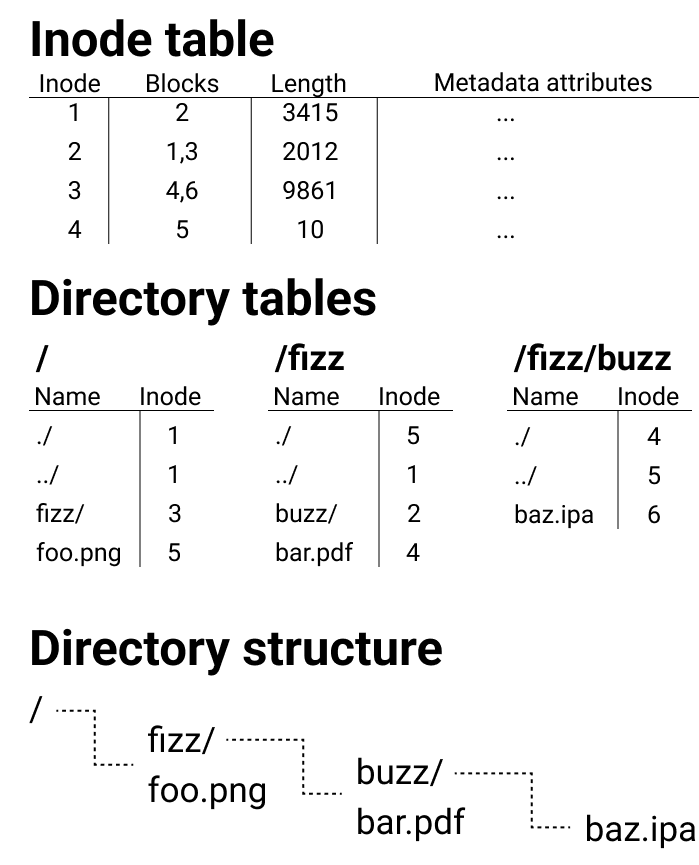
\includegraphics[width=0.5\textwidth]{figures/inode_diagram.png}
	\end{center}
	\caption{Basic structure of inode-based filesystem}
	\label{fig:inode_diag}
\end{figure}

\begin{minipage}{\linewidth}
\begin{lstlisting}[language=c, caption={Pseudocode of a minimalistic inode filesystem structure}, label=lst:inode_fs]
struct inode_entry {
	int 	length
	int[]	blocks
	// Metadata attributes are defined here
}

struct directory_entry {
	char*   filename
	int     inode
}

// Maps inode_id to a inode_entry
map<int, inode_entry> inode_table

\end{lstlisting}
\end{minipage}

Different filesystems provide different features and limitations. The Extended Filesystem (ext) exists in four different versions: ext, ext2, ext3, and ext4. This filesystem is often used on Unix systems. Each iteration brings new features and changes the limitations. For instance, comparing the two latest iterations, ext3 and ext4, ext4 can theoretically store files up to \SI{16}{\tebi\byte} while ext3 can store files up to \SI{2}{\tebi\byte}\,\cite{salterUnderstandingLinuxFilesystems2018}. Additionally, ext4 supports timestamps in units of nanoseconds while et3 only supports timestamps with a resolution of one second. Additionally. ext4 natively supports encryption at the directory level through the use of the fscrypt API\,\cite{FscryptArchWiki}.

The Apple Filesystem (APFS) is a modern filesystem that is used on iPhones and Mac and can store files with a size up to \SI{9}{\exa\byte}\,\cite{igotofferAPFSAppleFile2017}. It supports timestamps in units of nanoseconds and is built to be used on solid-state drives (SSD)\,\cite{nelsonWhatAPFSDoes}. It also supports modern features that its predecessor Mac OS Extended (HFS+) does not support, such as Snapshots and Space Sharing. APFS natively supports encryption of the filesystem volume\,\cite{appleinc.FileSystemFormats}.

\subsection{Distributed filesystems}
Filesystems are used to store data, for instance locally on a hard drive of a computer, or in the cloud. Google Drive is an example of a filesystem that enables users to save their data online with up to \SI{15}{\giga\byte} for free\,\cite{CloudStorageWork} using Google's clusters of distributed storage devices, meaning that the data is saved on Google's servers which can be located wherever they have data centers\,\cite{DistributedStorageWhat}. Paying customers can have a greater amount of storage using the service. Apple's iCloud and Microsoft's OneDrive are two additional examples of distributed filesystems where users have the option of free-tier and paid-tier storage.

Cloud-based filesystems, as opposed to a filesystem on a physical disk, are accessible from multiple computers and devices without requiring the user to connect a physical disk to the computer. Instead, as the filesystem is accessible through the internet, it can be accessed regardless of the user's location and on multiple devices, as long as a connection to the filesystem can be established. Thus, even if the user would lose their computer or if it would malfunction, the data on the cloud-based filesystem can still be accessed which means that the data could still be recovered. These filesystems are often owned by companies, such as Google Drive and Apple's iCloud, as they are big companies that can provide reliable storage. This also means that they have their own agenda and policies, and as they are hosting the data they have the possibility of accessing your data. The data is often encrypted, but in the case of Google Drive they have access and control of the encryption and decryption keys which in turn means that they have access and control of the data stored\,\cite{johnsonGoogleDriveSecure2021}. While they mention in their Terms of Service that the user retains ownership of the data\,\cite{googleGoogleDriveTerms}, they also mention that they can disclose your data for legal reasons and that they retain the right to review the content uploaded by users\,\cite{googleGoogleTermsService}. By them controlling the encryption and decryption keys, it also enables the possibility of hackers gaining access to your data by attacking Google. iCloud uses end-to-end encryption for some parts of the service, but not for the whole suit\,\cite{appleinc.ICloudSecurityOverview}. For instance, backup data and iCloud drive is not end-to-end encrypted while the Keychain and Memoji data is.

\subsection{Data storage and encoding}
\label{sec:data_storage}
Different file types have different protocols and definitions of how they should be encoded and decoded, for instance, a JPEG and a PNG file can be used to display similar content but the data they store is different. At the lowest level, storage devices often represent files as a string of binary digits no matter the file type (however there are non-binary storage devices\,\cite{MultistateDataStorage2020}, but this is outside the scope of this thesis). If one would represent an arbitrary file of $X$ bytes, each byte (0x00 - 0xFF) can be represented as a character such as the Extended ASCII (EASCII) keyset and we can therefore decode this file as $X$ different characters. Using the same set of characters for encoding and decoding we can get a symmetric relation for representing a file as a string of characters. EASCII is only one example of such a set of characters, any set of strings with $256$ unique symbols can be used to create such a symmetric relation, for instance, $256$ different emojis or a list of $256$ different words. However, if we are using a set of words we would also have to introduce a unique separator so that the words can be distinguished. If we would use a single space character as the separator, we could make the encoded text look like a text document; however, random words one after another lead to a high probability of creating an unstructured text document. Further, if punctuation is introduced, for instance as part of some words, the text document could look like it contains random and unstructured sentences.

This string of $X$ bytes can also be used as the data in an image. An image can be abstracted as a $h * w$ matrix, where each element is a pixel of a certain color. In an image with 16-bit Red-Green-Blue (RGB) color depth, each pixel consists of three 16-bit values, i.e. three pairs of bytes. One can therefore imagine that we can use this string of $X$ bytes to assign colors in this pixel matrix by assigning the first two bytes as the first pixel's red color, the next two bytes as the same pixel's color green color, and so forth. The seventh and eight byte would represent the second pixels red color. This means that $X$ bytes of data can be represented as 
$$ceil(\frac{X}{2 * 3})$$ 
pixels, where $ceil$ rounds a float to the closest larger integer. For a file of \SI{1}{\mega\byte}, i.e. $X = 1\,000\,000$ we need $166\,667$ pixels in an image with 16-bit RGB color depth. The values of $h$ and $w$ are arbitrary but if we for instance want a square image we can set $ h\,=\,w\,=\,409$ which means that there will be $167\,281$ pixels in total, and the remaining $614$ pixels will just be fillers to make the image a reasonable size. Using filler pixels requires us to keep track of the number of bytes that we store in the image so that we do not read the filler bytes when the image is decoded. However, we could choose $h = 1$ and $w = 166\,667$ which would mean a very wide image but would not require filler pixels. 

This means that we can represent any file as a string of bytes which can then be encoded into text or as an image, which can be posted on for instance social media. However, there is a possibility that the social media services compress the images uploaded which could lead to data loss in the image, which would mean that the decoded data would be different from the encoded data. In this case, we would not be able to retrieve the original data that was stored unless we would use methods such as error correcting codes.